%#!platex
% NLP2026 サンプル文書．パブリックドメイン．
\documentclass[
  platex, dvipdfmx,  % ワークフローは必ず明示的に指定する
]{nlp2026}
%english option
%\documentclass[platex, dvipdfmx, english]{nlp2026}
%#!uplatex
%\documentclass[uplatex,dvipdfmx]{nlp2026}
%#!lualatex
%\documentclass[lualatex]{nlp2026}


% パッケージ
\usepackage{graphicx,xcolor}  % グラフィックス関連
\usepackage{url}

% 以下は(u)pLaTeX用．LuaLaTeX使用時には削除すること
\usepackage[T1]{fontenc}      % モダンなフォントエンコーディング
\usepackage{jlreq-deluxe}     % 多書体化（otf パッケージは使用しない）
\usepackage{pxrubrica}        % ルビ

%% option 不要な場合はコメントアウト
%\usepackage{bxjalipsum}       % ダミーテキスト（最終版では削除）
\usepackage{hyperref}
\hypersetup{
	colorlinks=true,
    citecolor=blue,
    linkcolor=blue,
    urlcolor=blue,
	pdfborder={0 0 0},
}
\usepackage[verb]{bxghost}    % \verb 前後に適切な和欧文間スペース
\usepackage{xurl}

% 参考文献のフォントサイズを指定
%\renewcommand{\bibfont}{\normalsize} % 標準サイズ
%\renewcommand{\bibfont}{\footnotesize} % より小さく

% \emph をゴシックかつ太字に（比較的新しい LaTeX が必要）
\DeclareEmphSequence{\gtfamily\sffamily\bfseries}

% 著者用マクロをここに入れる
\newcommand{\pkg}[1]{\textsf{#1}}
\newcommand{\code}[1]{\texttt{#1}}
\newcommand{\comment}[1]{\textcolor{red}{#1}}
%%%%%%%


\title{LLM-jp FT-LLMコンペにおける\\数学推論能力向上の取り組み}

\author{%
  尾崎 大晟${}^{1}$ \quad
  力岡 友和${}^{1}$ \quad
  渡部 泰樹${}^{1}$ \quad
  Jeong~Seong~Cheol${}^{2}$\\[4pt]
  ${}^{1}$ 株式会社松尾研究所\
  ${}^{2}$ 東京大学 松尾・岩澤研究室
}

\begin{document}

\maketitle
\begin{abstract}
本稿では，LLM-jp FT-LLMコンペティションにおける我々のチームの取り組みを報告する．
本コンペティションでは，llm-jp-4-8bをベースモデルとし，中学校・高等学校レベルの数学問題に対する正答率を競う．
我々は，(1) YaRNによるコンテキスト長拡張，(2) gpt-oss-120bを活用した合成推論データの構築，(3) SFTおよびGRPOによる学習，の3つを組み合わせた．
特にデータ合成では，GSM8KおよびStackMathQAを基にChain-of-Thought（CoT）とTool-Integrated Reasoning（TIR）の2種類の推論データを生成し，LLM-as-a-Judgeによる多段階品質管理を行った．
\end{abstract}

%=============================================================
\section{はじめに}
%=============================================================

LLM-jp FT-LLMコンペティション\cite{ftllm2026}は，llm-jpが主催するLLMファインチューニングの公開コンペティションである．
参加チームはllm-jp-4-8bをベースモデルとして，日本の中学校・高等学校レベルの数学問題500問に対する正答率を競う．
推論時にはllm-jp-4-8bをベースとしたモデルのみ使用可能であり，外部LLMの利用やインターネットアクセスは禁止されている．

我々のチームでは，以下の3つの戦略を組み合わせた．
\begin{enumerate}
\item \textbf{コンテキスト長の拡張:} YaRN\cite{yarn}により，長い推論過程を扱えるようコンテキスト長を拡張する
\item \textbf{合成推論データの構築:} gpt-oss-120bを用いてCoTおよびTIRの推論データを合成し，多段階の品質管理を行う
\item \textbf{SFTおよびGRPO:} 合成データを用いた教師ありファインチューニングとGRPOによる強化学習を実施する
\end{enumerate}

以下，第\ref{sec:baseline}節で予備調査とコンテキスト長拡張について，第\ref{sec:synth}節で合成推論データの構築について，第\ref{sec:sft_rl}節でSFTおよびGRPOについて，第\ref{sec:inference}節で推論パイプラインについて述べる．

%=============================================================
\section{予備調査とコンテキスト長拡張}
\label{sec:baseline}
\label{sec:context}
%=============================================================

本節では，ベースモデルllm-jp-4-8bの推論能力を把握するための予備実験と，コンテキスト長拡張について述べる．

\subsection{ベースライン実験}

コンペティションで配布されたテストデータに対して評価を行ったところ，単純な指示文のみのプロンプトでは正答率は0.08に留まった．一方，SFTで使用するプロンプト形式（指示・入力・応答）に揃えることで正答率は0.32まで改善し，さらに英語プロンプトを用いることで0.40まで向上した．
この結果から，推論性能はプロンプト設計および使用言語に大きく依存することが確認された．
比較のため大規模モデルも評価し，\texttt{gpt-oss-120b}では0.81，\texttt{Qwen3-235B-A22B-Thinking}では0.74の正答率を得た．

\subsection{コンテキスト長の拡張}

数学問題の推論では長いChain-of-Thought推論過程を生成する必要があるため，YaRN (Yet another RoPE extensioN)\cite{yarn}によりベースモデルのコンテキスト長を拡張した．


%=============================================================
\section{合成推論データの構築}
\label{sec:synth}
%=============================================================

本節では，SFTに用いる合成推論データの生成パイプラインについて述べる．
パイプラインのソースコードは公開されている\footnote{\url{https://github.com/ft-llm-team-mkj/synthetic-data-pipeline}}．

\subsection{パイプライン概要}

本パイプラインは，既存の数学QAデータセットを入力とし，高品質な推論過程を付与したSFT用データセットを出力する．
処理は大きく3段階からなる: (1) データソースの前処理，(2) CoT/TIR推論の生成，(3) 多段階品質検証．

\subsection{データソースと前処理}

データソースとしてGSM8K\cite{gsm8k}およびStackMathQA\cite{stackmathqa}を用いた．

\paragraph{GSM8K}
GSM8Kは小学校レベルの算数文章題約8,500問からなるデータセットである．
各問題の回答に含まれる「\code{\#\#\#\#}」マーカー以降を最終回答として抽出した．

\paragraph{StackMathQA}
StackMathQAはStack Exchangeの数学関連Q\&Aを収集したデータセットである．
前処理として，(1) 1問あたりの回答数が5以下，(2) 回答テキストの長さが3,000文字以下のフィルタリングを適用し，30,000件をサンプリングした．
複数回答がある場合は，gpt-oss-120bにより最適な回答を選定し，質問文の簡潔化も行った．


\subsection{CoT拡張}

各QAペアに対し，問題から回答に至るChain-of-Thought推論過程を生成した．
多様性を確保するため各問題につき3候補を生成した．

生成された候補はLLM-as-a-Judge方式で評価した．
評価基準は直接性（30\%），明瞭性（30\%），完全性（20\%），効率性（20\%）の4項目（各1〜10点）であり，重み付き総合スコアを算出する．
3候補中の最高スコア候補を選択し，後段の品質検証（第\ref{sec:quality}節）で総合スコア$\geq$7のフィルタリングを適用した．

\subsection{TIR拡張}

CoT拡張に加え，Tool-Integrated Reasoning（TIR）データも生成した．
TIRでは，推論過程に加えて実行可能なPythonコードを\code{<tool\_call>}タグで付与する．
CoTと同様に3候補を生成し，LLM-as-a-Judgeによりコード正確性，推論明瞭性，完全性の3項目（各1〜10点）で評価し，最高スコア候補を選択した．

TIRデータに対しては後処理として以下の2段階の検証を実施した:
\begin{enumerate}
\item \textbf{実行検証}: Pythonサンドボックス経由でコードを実行し，エラーなく動作するかを確認
\item \textbf{意味的一致検証}: 実行結果と期待回答の意味的一致をLLMで評価（数値フォーマットや単位の差異を許容）
\end{enumerate}

\subsection{品質管理とマージ}
\label{sec:quality}

生成段階で最良候補を選択した後，後処理として品質の再評価を行った．
CoTデータに対しては，生成時と同じ4基準（直接性・明瞭性・完全性・効率性）でLLMによる品質再評価を実施し，総合スコア$\geq$7のデータのみを有効とした．
TIRデータに対しては，前述の2段階検証に加え，コード正確性と推論明瞭性の平均スコア$\geq$7を有効条件とした．

生成されたデータセットはHuggingFace Hub上に公開している\footnote{\url{https://huggingface.co/datasets/ft-llm-team-mkj/cot-merged}}．

%=============================================================
\section{SFTおよびGRPO}
\label{sec:sft_rl}
%=============================================================

第\ref{sec:synth}節で構築した合成データを用いて，教師ありファインチューニング（SFT）およびGRPO（Group Relative Policy Optimization）\cite{grpo}による強化学習を実施した．
学習基盤にはNVIDIAのNeMo-RL\cite{nemorl}を採用した．
NeMo-RLはRayベースの分散学習フレームワークであり，DTensorによるモデル並列化とvLLM\cite{vllm}による高速な推論生成を，同一GPU上で時分割（colocated mode）により実現する．

\subsection{SFT}

第\ref{sec:synth}節のパイプラインで生成したCoTデータ（訓練33,905件，検証1,784件）を用いてSFTを実施した．
データは\code{<think>}タグ付きのCoT推論を含むOpenAIチャット形式である．
YaRNにより8k/16k/32kの3種類のコンテキスト長拡張を行ったが，32kでも計算リソースに十分な余裕があったため，最終的に32kバリアントを採用した．
SFTデータの系列長が最大でも8,192トークンに収まったため，SFTでは最大系列長を8,192トークンに設定して学習を行った．

主要なハイパーパラメータを表\ref{tab:sft}に示す．
DTensorによるテンソル並列（TP=2）とactivation checkpointingを有効化し，8基のH100 GPUを用いた．
Sequence packingにより異なる長さの系列を効率的にバッチ化し，GPU利用率を向上させた．
チェックポイントは検証損失に基づき上位3つを保存した．

図\ref{fig:sft_loss}にSFTの訓練損失の推移を示す．
損失は学習初期に急速に低下し約0.55に収束した後，3エポック目の終盤でさらに0.4付近まで低下した．

\begin{figure}[t]
\centering
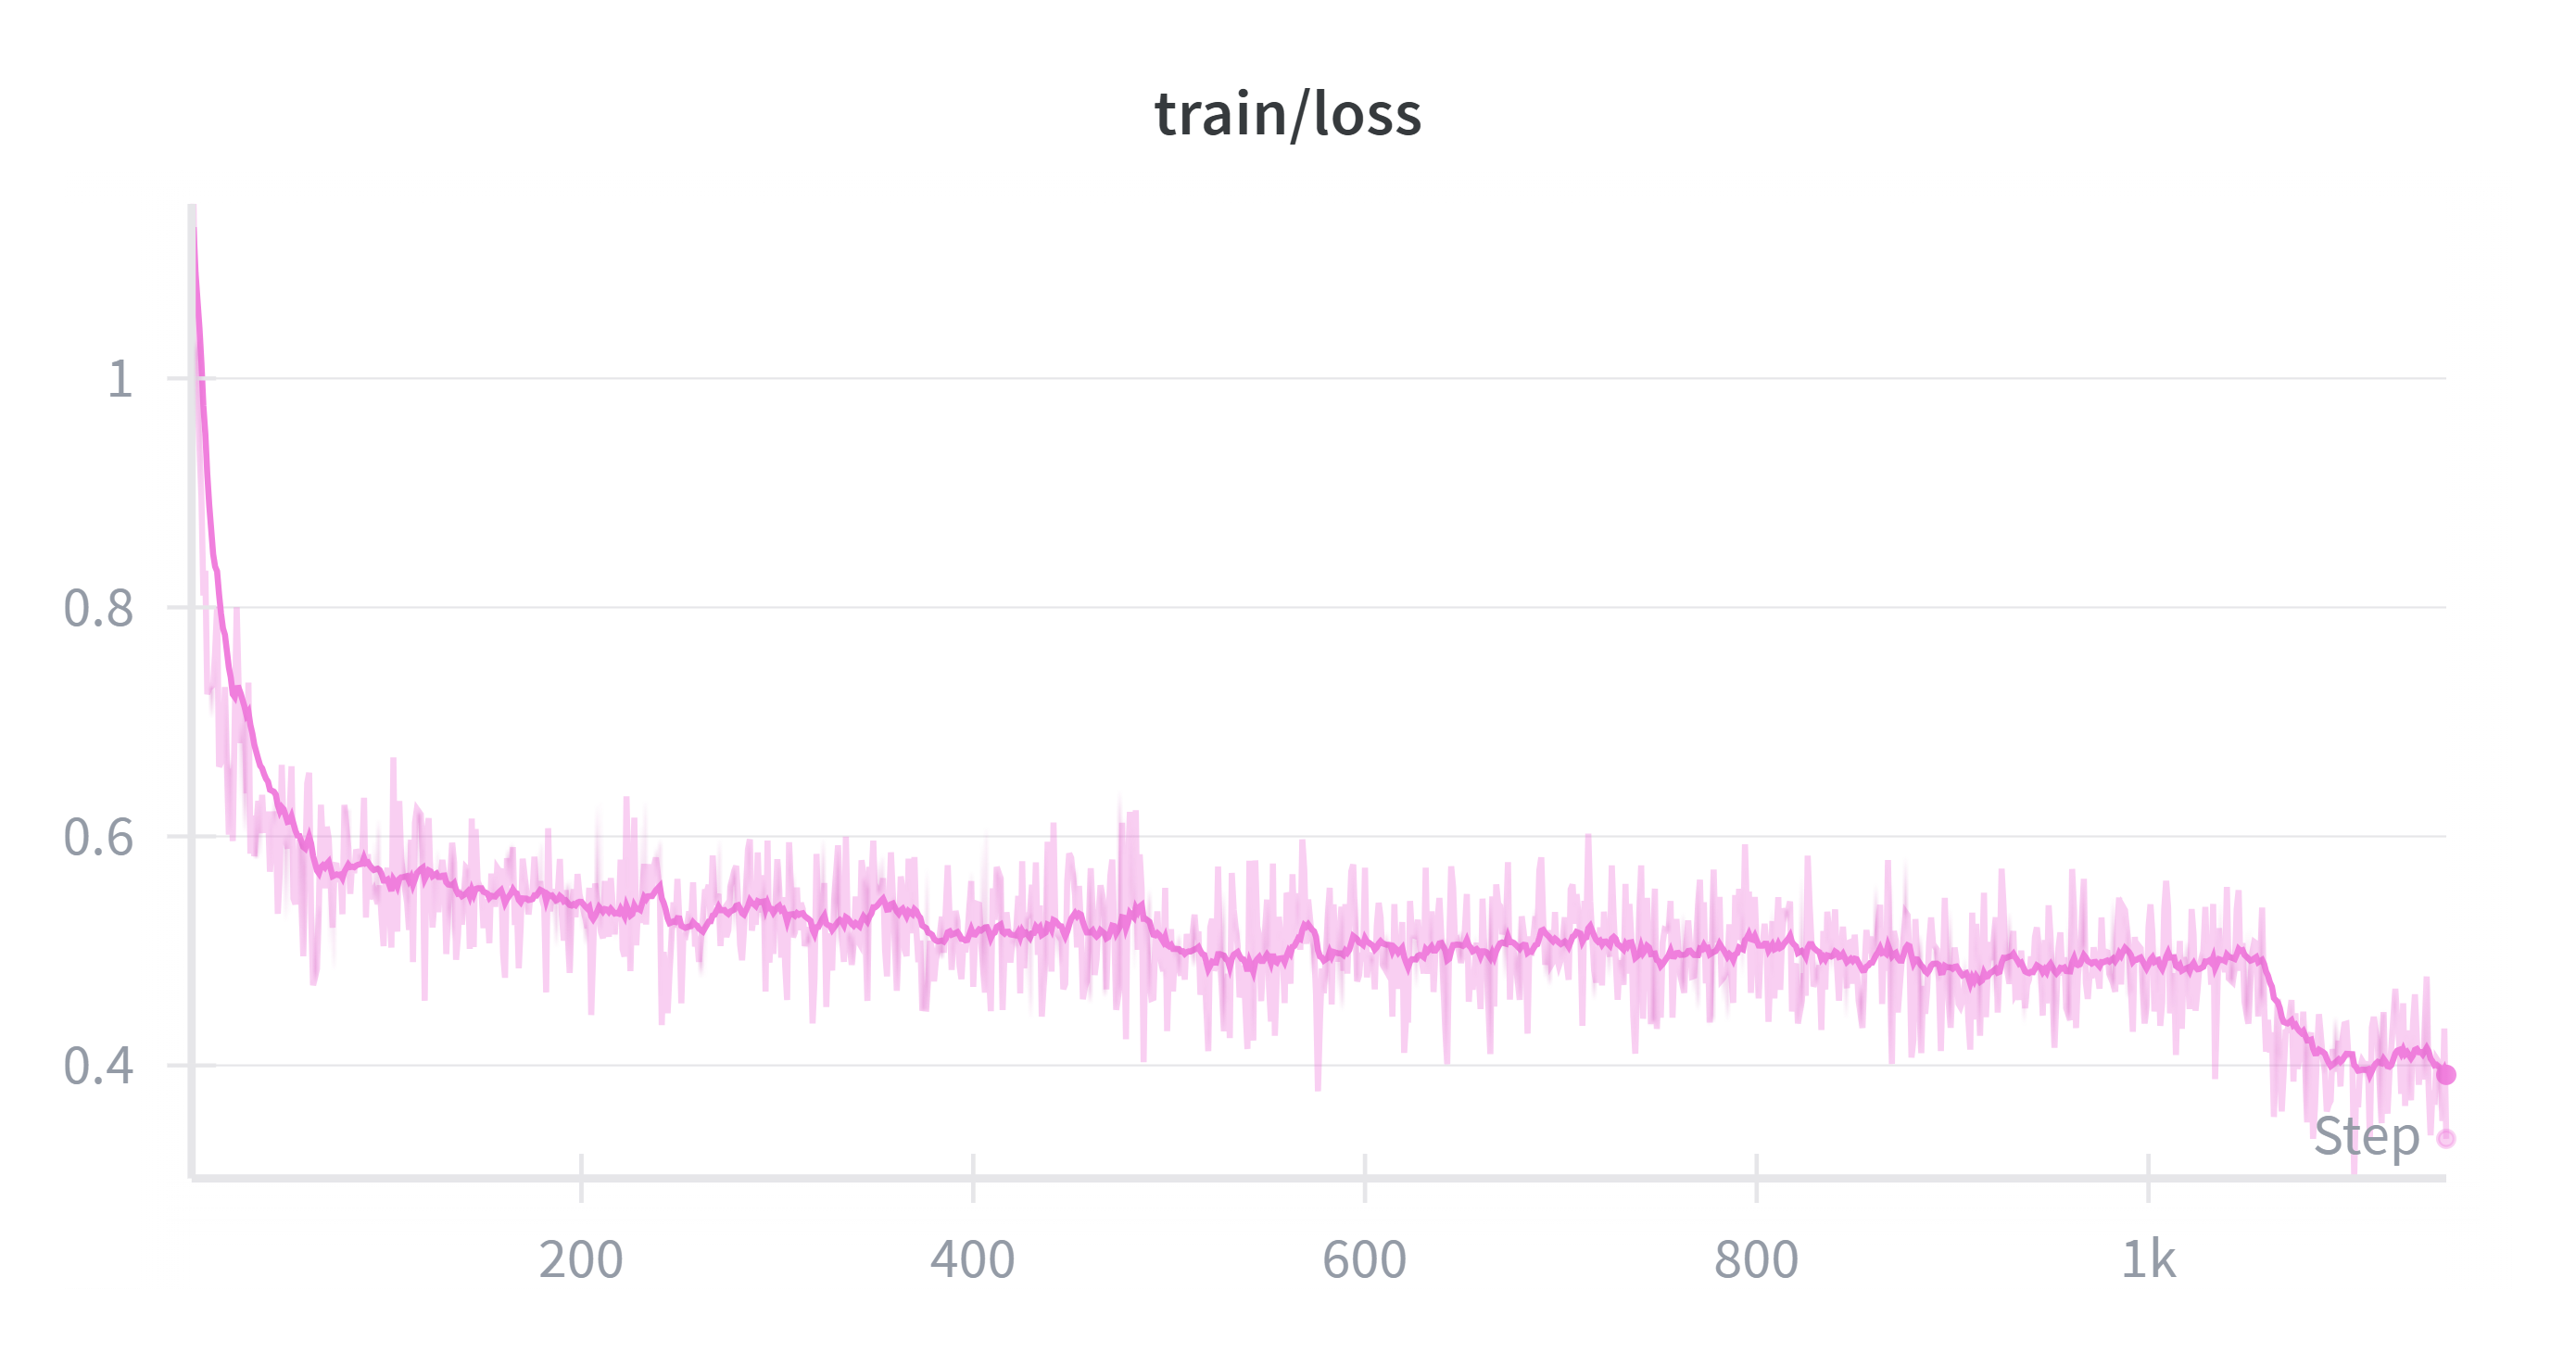
\includegraphics[width=\linewidth]{sft_loss.png}
\caption{SFTにおける訓練損失の推移}
\label{fig:sft_loss}
\end{figure}

\begin{table}[t]
\centering
\caption{SFTの主要ハイパーパラメータ}
\label{tab:sft}
\small
\begin{tabular}{ll}
\hline
\textbf{項目} & \textbf{値} \\
\hline
GPU & H100 $\times$ 8（1ノード） \\
精度 & bfloat16 \\
テンソル並列（TP） & 2 \\
エポック数 & 3 \\
グローバルバッチサイズ & 32 \\
最適化手法 & AdamW \\
学習率 & $2 \times 10^{-5}$ \\
$(\beta_1, \beta_2)$ & $(0.9, 0.98)$ \\
重み減衰 & 0.1 \\
勾配クリッピング & 1.0 \\
Sequence packing & 有効（MFFD） \\
\hline
\end{tabular}
\end{table}

\subsection{GRPO}

SFTで得られたチェックポイントを初期方策とし，GRPOによる強化学習を実施した．
GRPOはプロンプトごとに複数の応答を生成し，グループ内の相対的な報酬に基づいて方策を更新するアルゴリズムである\cite{grpo}．
学習データとして数学問題180件（検証20件）を用い，SFTよりも長い推論生成を許容するため最大系列長を16,384トークンに拡張して最大600ステップの学習を行った．

\paragraph{報酬設計}
報酬関数は，バイナリ正誤判定とLLMによる部分点の2段構成とした．
まずhf\_math\_verifyによりモデル出力の最終回答を正誤判定する．
正解の場合は報酬1.0を付与し，不正解の場合はgpt-oss-120bによる推論過程の評価に基づき部分点を付与する．
部分点はLLMスコア（0〜1）に重み$\alpha = 0.2$を乗じた値とした:
\begin{equation}
r = \begin{cases}
1.0 & \text{(正解)} \\
\alpha \cdot r_{\text{LLM}} & \text{(不正解)}
\end{cases}
\end{equation}
この設計により，最終回答が誤りであっても推論過程が適切であれば勾配情報が得られ，学習の安定化に寄与する．

\paragraph{学習設定}
NeMo-RLのcolocated modeを用い，DTensorによる学習（TP=2）とvLLMによる生成（TP=1，各GPU独立）を同一の8基のH100上で時分割実行した．
主要なハイパーパラメータを表\ref{tab:grpo}に示す．
Leave-one-out baselineによる分散低減と，応答が最大長を超過した場合のペナルティ（reward shaping）を適用した．
参照方策とのKLダイバージェンスにはk3推定量\cite{k3kl}を用い，係数$\beta = 0.01$で正則化した．

図\ref{fig:grpo_reward}にGRPOの訓練報酬の推移を示す．
報酬は学習開始時の約0.55から単調に増加し，600ステップで約0.9に達した．
また，図\ref{fig:grpo_gen_tokens}に生成トークン数の推移を示す．
学習の進行に伴い平均生成トークン数は約390から約340へ減少しており，モデルがより簡潔な推論で正解に到達できるようになったことが示唆される．
なお，生成トークン数は終始500トークン以下で推移しており，16,384トークンの最大系列長は過剰であった可能性がある．

\begin{figure}[t]
\centering
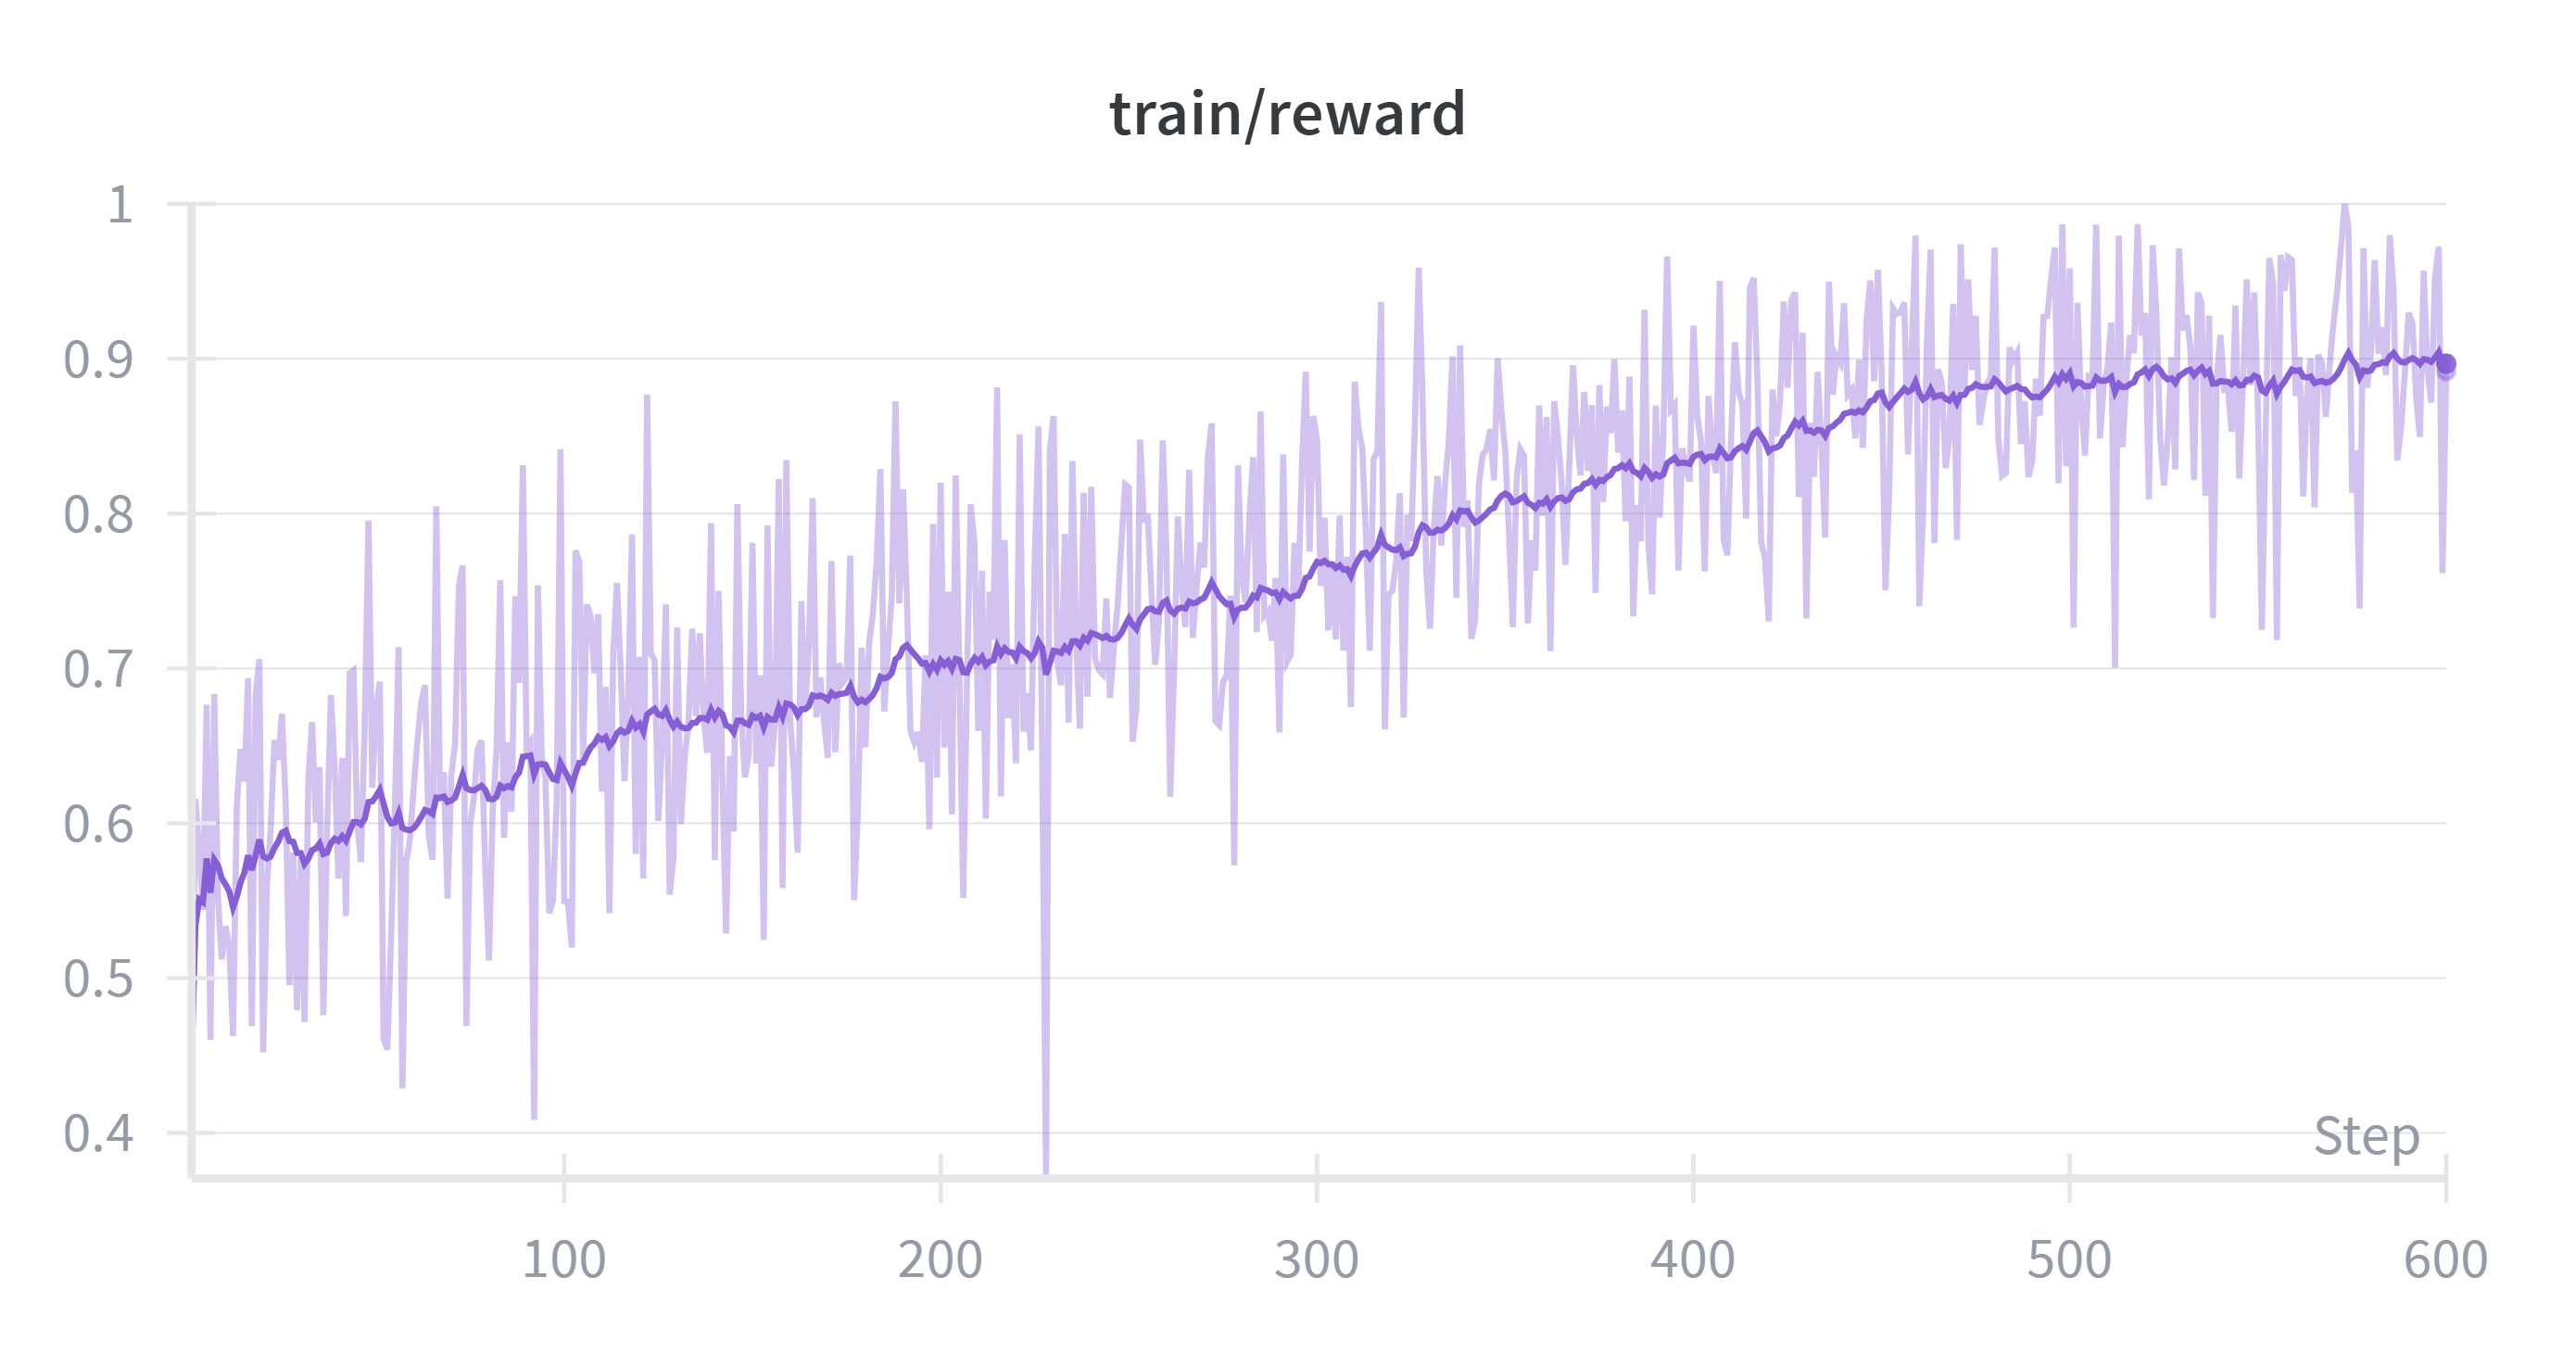
\includegraphics[width=\linewidth]{reward.png}
\caption{GRPOにおける訓練報酬の推移}
\label{fig:grpo_reward}
\end{figure}

\begin{figure}[t]
\centering
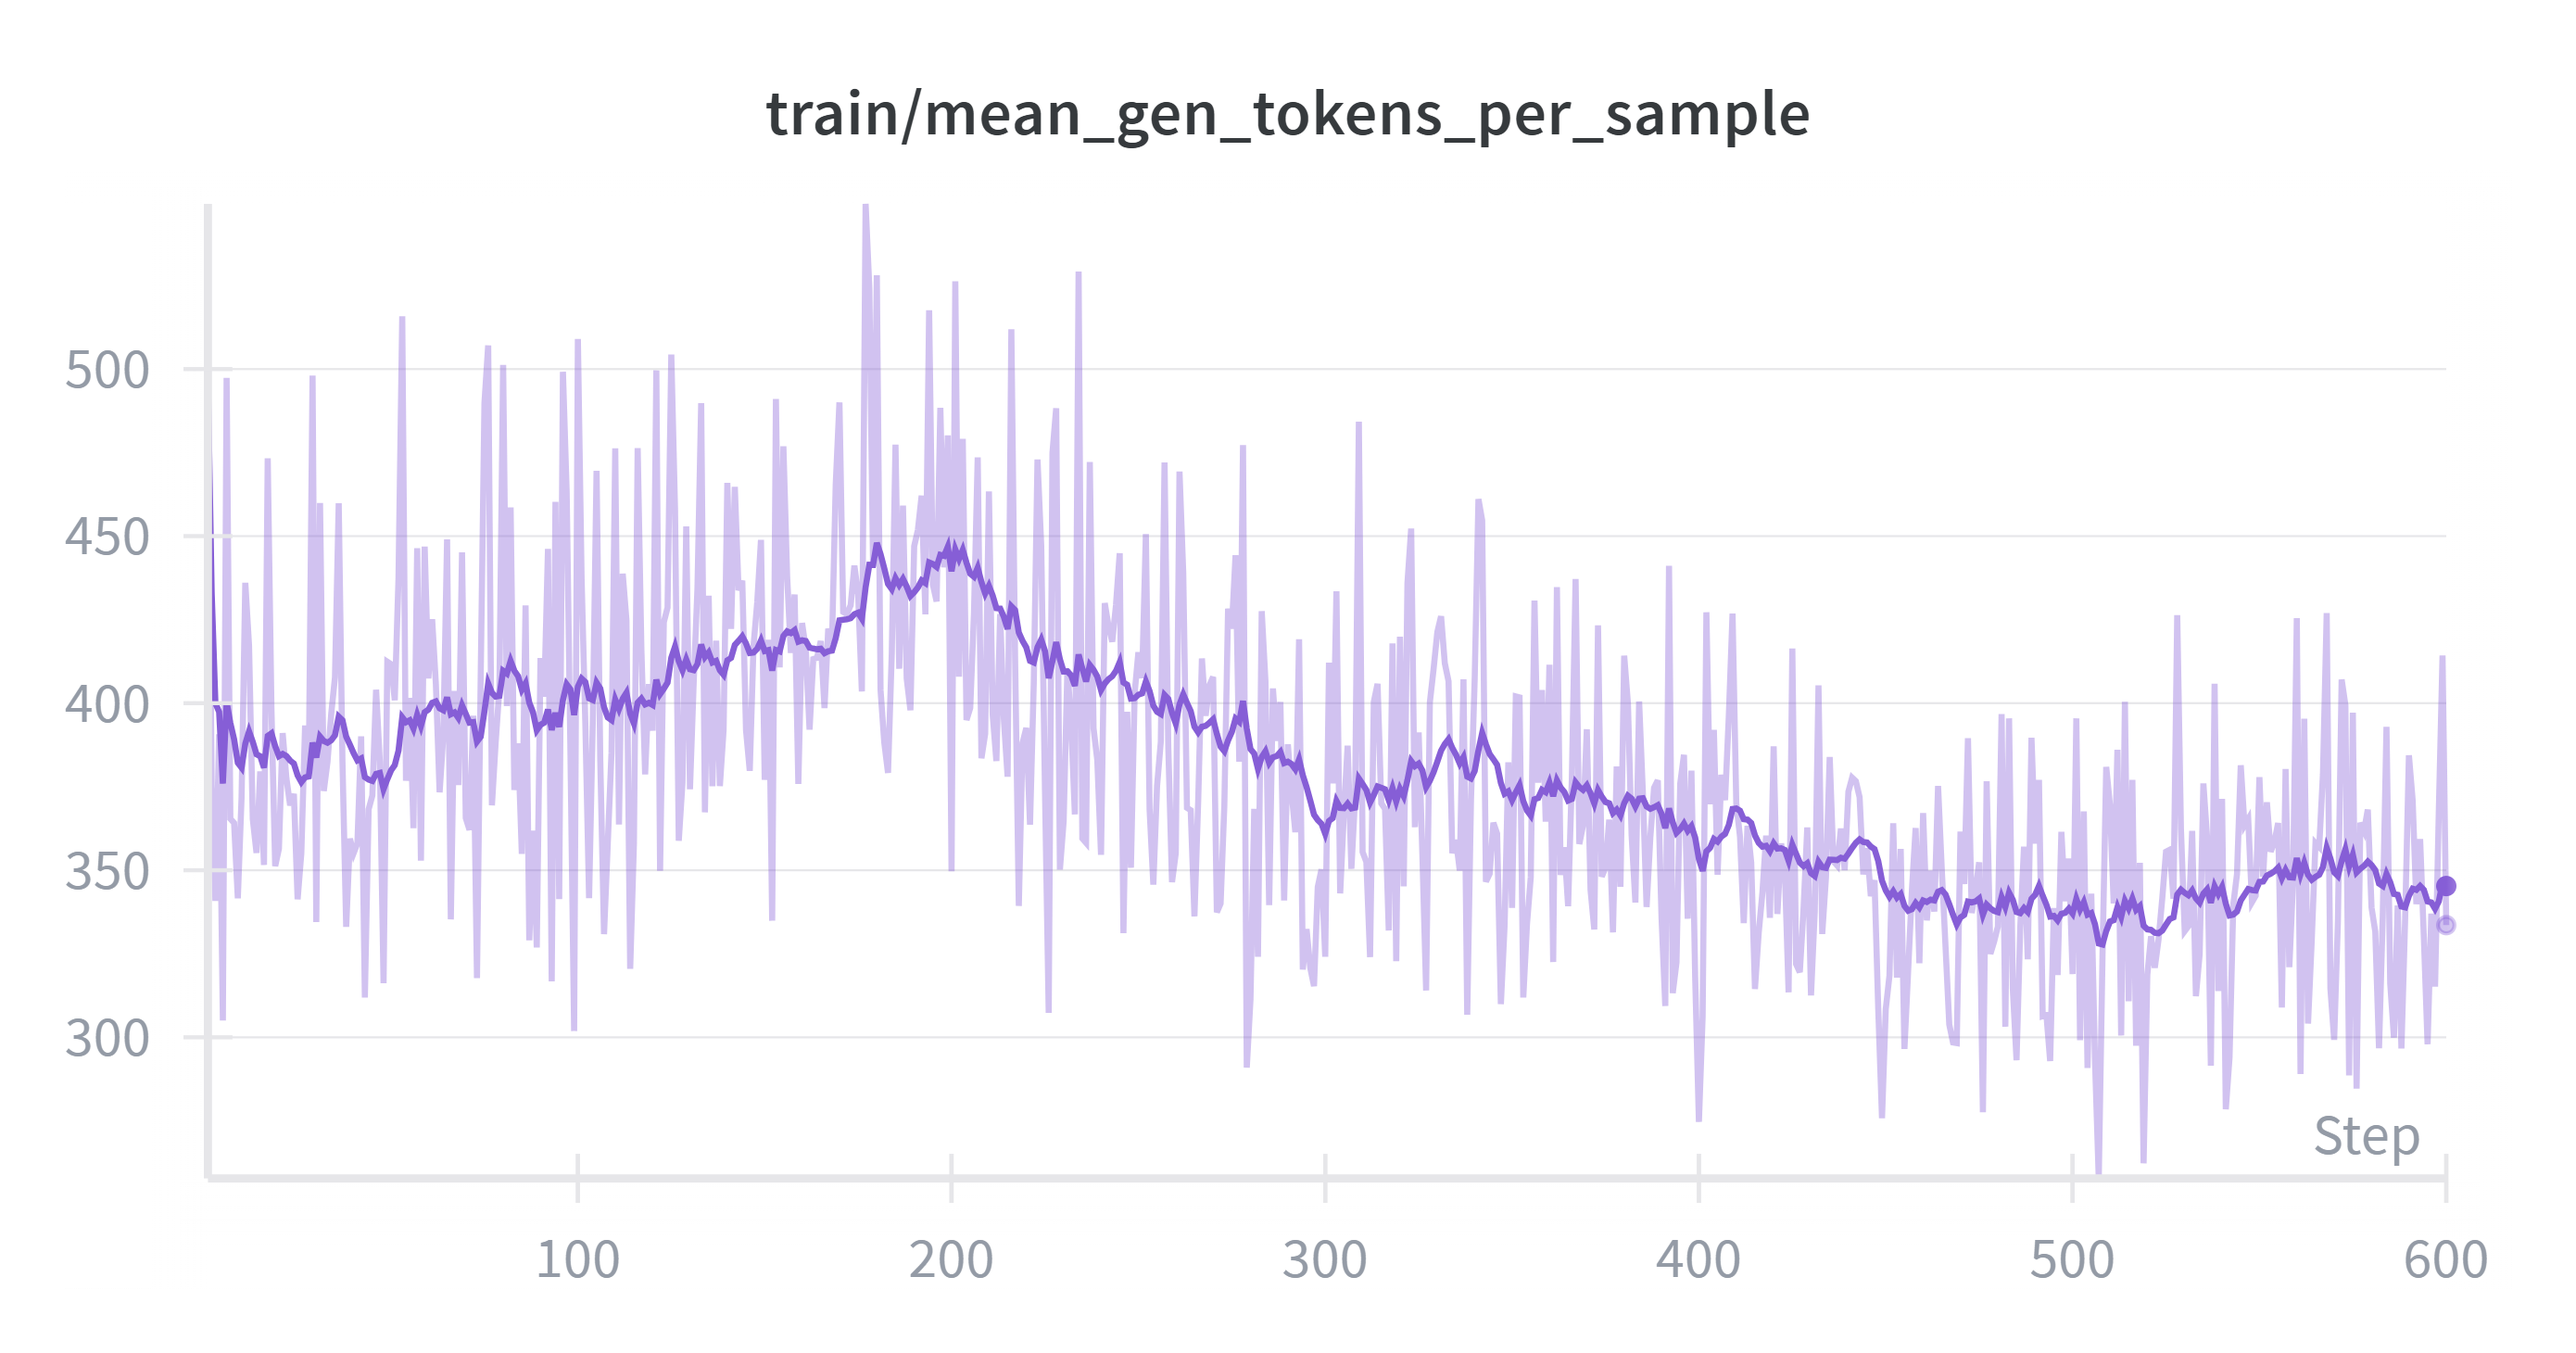
\includegraphics[width=\linewidth]{grpo_gen_token.png}
\caption{GRPOにおける平均生成トークン数の推移}
\label{fig:grpo_gen_tokens}
\end{figure}

\begin{table}[t]
\centering
\caption{GRPOの主要ハイパーパラメータ}
\label{tab:grpo}
\small
\begin{tabular}{ll}
\hline
\textbf{項目} & \textbf{値} \\
\hline
GPU & H100 $\times$ 8（1ノード） \\
精度 & bfloat16 \\
プロンプト数/ステップ & 16 \\
生成数/プロンプト & 8 \\
最大ステップ数 & 600 \\
生成温度 & 0.7 \\
学習率 & $1 \times 10^{-6}$ \\
$(\beta_1, \beta_2)$ & $(0.9, 0.999)$ \\
重み減衰 & 0.01 \\
PPOクリップ $\epsilon$ & 0.2 \\
KL係数 $\beta$ & 0.01 \\
報酬正規化 & 有効 \\
LLM部分点重み $\alpha$ & 0.2 \\
\hline
\end{tabular}
\end{table}

%=============================================================
\section{推論パイプライン}
\label{sec:inference}
%=============================================================

推論パイプラインは，(1) 問題の日英翻訳，(2) マルチエージェント並列推論，(3) 回答抽出と多数決投票の3段階からなる．
推論エンジンにはvLLMを使用し，8基のGPU上で並列に実行する．
なお，第\ref{sec:synth}節で述べたTIRデータは学習してみたが，学習後のモデルにおいてPythonコードの生成が安定しなかったため，最終的な推論パイプラインではCoTベースの推論のみを採用した．

\subsection{問題の日英翻訳}

入力された日本語の数学問題を，まずSFTで構築した翻訳モデル（math-translator\_v2\footnote{\url{https://huggingface.co/ft-llm-team-mkj/math-translator_v2}}）により英語に変換する．
各問題に対して4つの翻訳候補を生成する．一部誤訳が含まれる可能性があるため，
複数の翻訳候補を生成することで，翻訳の多様性を確保し，後段の推論における回答の多様性を高める．
英語への変換を導入した動機は，ベースモデルllm-jp-4-8bの事前学習データにおいて英語の比率が高く，英語の数学問題に対してより高い推論性能を発揮すると期待されるためである．

\subsection{マルチエージェント並列推論}

翻訳された問題に対し，8つの独立した推論エージェントをマルチプロセスにより並列に起動する．
モデルの割り当てはエージェントごとに異なり，エージェント0--5にはmath-reasoner-v2\footnote{\url{https://huggingface.co/ft-llm-team-mkj/math-reasoner-v2}}を，エージェント6--7にはmath-reasoner-v5\footnote{\url{https://huggingface.co/ft-llm-team-mkj/math-reasoner-v5}}を使用する．
math-reasoner-v2は幅広い難易度の問題でGRPOを適用したモデルであり，math-reasoner-v5は高難易度問題に特化してGRPOを適用したモデルである．
2種類のモデルを混在させることで，アンサンブル効果による回答精度の向上を狙った．

各エージェントは，全翻訳候補（1問あたり4候補）に対して5サンプルずつ推論を実行する．
したがって，1問あたり$4\text{（翻訳候補）} \times 8\text{（エージェント）} \times 5\text{（サンプル）} = 160$個の回答候補が得られる．
推論時の最大コンテキスト長は16,384トークンとし，第\ref{sec:context}節で述べたYaRNによる拡張を適用している．
これにより，長いChain-of-Thought推論過程を途中で打ち切ることなく生成できる．

\subsection{回答抽出と多数決投票}

各エージェントの出力から最終回答を抽出する．
モデルは\code{<think>}タグ内にChain-of-Thought推論過程を生成するため，\code{</think>}タグ以降のテキストを最終回答として取り出す．

抽出された160個の回答候補に対して多数決投票を行い，最終回答を決定する．
単純な文字列一致ではなく，math-verifyライブラリを用いた数学的等価性判定に基づくグルーピングを行う．
具体的には，新たな回答候補を既存の全グループの代表回答と比較し，数学的に等価なグループが存在すればそこに分類する．
最終的に，最大グループに属する回答の代表値を最終回答として出力する．

以上の推論パイプラインにより，テストデータにおける最終的な正答率0.70を達成した．

%=============================================================
\section{おわりに}
%=============================================================

本稿では，LLM-jp FT-LLMコンペティションにおける我々のチームの取り組みを報告した．
YaRNによるコンテキスト長拡張，合成データによるSFT，GRPOによる強化学習を組み合わせ，8Bパラメータモデルでの数学推論能力の向上を目指した．
データ合成パイプラインでは，CoTおよびTIRの2種類の推論データを生成し，LLM-as-a-Judgeとコード実行検証を組み合わせた多段階品質管理により，高品質なSFTデータを構築した．
一方で，TIRデータは学習に用いたものの，推論時のコード生成が安定しなかったため最終的な推論パイプラインには採用しなかった．

今後の課題として，GRPOの学習安定化，より多様なデータソースの活用，および推論時におけるTool Use統合の実現が挙げられる．


%%%%  ここまでが本文　4ページ以内
\newpage
\section*{謝辞}
本取り組みはLLM-jpコミュニティおよびABCI 3.0の計算資源の提供を受けて実施された．関係者の皆様に感謝申し上げる．


% 参考文献
\bibliographystyle{junsrt}
\bibliography{ftllm_refs}

%%%%  ここまでが本文+参考文献　5ページ以内


% 付録(Appendix)
\clearpage
\appendix
\section{付録}
\label{sec:rl}

本付録では，本コンペティションにおいて検討したアプローチのうち不採用としたLooped Transformerと，YaRNおよびコンテキストウインドウに関する追加実験について報告する．

\subsection{Looped Transformer}

Looped Transformerは，同一のTransformerブロックを$N$回ループさせることで実効的な深さを拡張するアーキテクチャである．
理論的には，ループ構造によりチューリング完全な計算が可能であること\cite{giannou2023looped}，通常のTransformerの10\%以下のパラメータ数で同等の性能を達成できること\cite{yang2024looped}，有利な損失景観の帰納バイアスを誘導すること\cite{fan2025looped_landscape}が示されている．

McLeish~ら\cite{mcleish2025retrofitting}は，事前学習済みLLMにループ構造を後付けする手法を提案し，1Bクラスのモデルで同一計算予算下で通常のpost-trainingを上回る数学推論性能を達成している．
しかし，既存の検証が1Bクラスに限られ8Bモデルへの適用可能性が不明確であること，高難度問題での効果が限定的であること，学習コストが高い（中規模実験で32 GPU規模）ことから，本コンペでは採用を見送った．

\subsection{YaRNの拡張度合いの影響}

YaRNのスケーリング係数がGRPO学習に与える影響を調べるため，コンテキスト長拡張を8k，16k，32kに設定した3条件でGRPOを実施した．
図\ref{fig:yarn_reward}に各条件の訓練報酬の推移を示す．
3条件の報酬曲線はほぼ一致しており，拡張度合いによる大きな差は見られなかった．
ただし，100ステップ以降では拡張度合いの大きい32kバリアントがわずかに高い報酬を示す傾向が見られた．
Ye~ら\cite{polaris}はYaRNの推論時適用により長文脈での精度が大幅に向上することを報告しており，YaRNの主たる効果は学習時よりも推論時のコンテキスト長外挿にあると考えられる．

\subsection{コンテキストウインドウサイズの影響}

GRPO学習時のコンテキストウインドウサイズの影響を調べるため，YaRN 16kモデルに対し，最大系列長を1k，2k，4k，8k，16kに変えた5条件でGRPOを実施した．
図\ref{fig:ctx_reward}に訓練報酬の推移を，図\ref{fig:ctx_length}に平均生成トークン数の推移を示す．
報酬の最終到達値はいずれの条件でもおおむね同程度であったが，1kの条件では学習初期（約100ステップまで）の報酬立ち上がりが他条件と比べて遅れる傾向が見られた．
一方，平均生成トークン数は全条件で500トークン以下で推移しており，本タスクでは2k以上のコンテキストウインドウがあれば十分であることが示唆される．
Ye~ら\cite{polaris}も，事前学習時のコンテキスト長を超える領域でのRL学習はサンプルの大部分が長文脈を活用せず効率が低いことを報告しており，本実験の結果もこの知見と整合的である．

\begin{figure}[t]
\centering
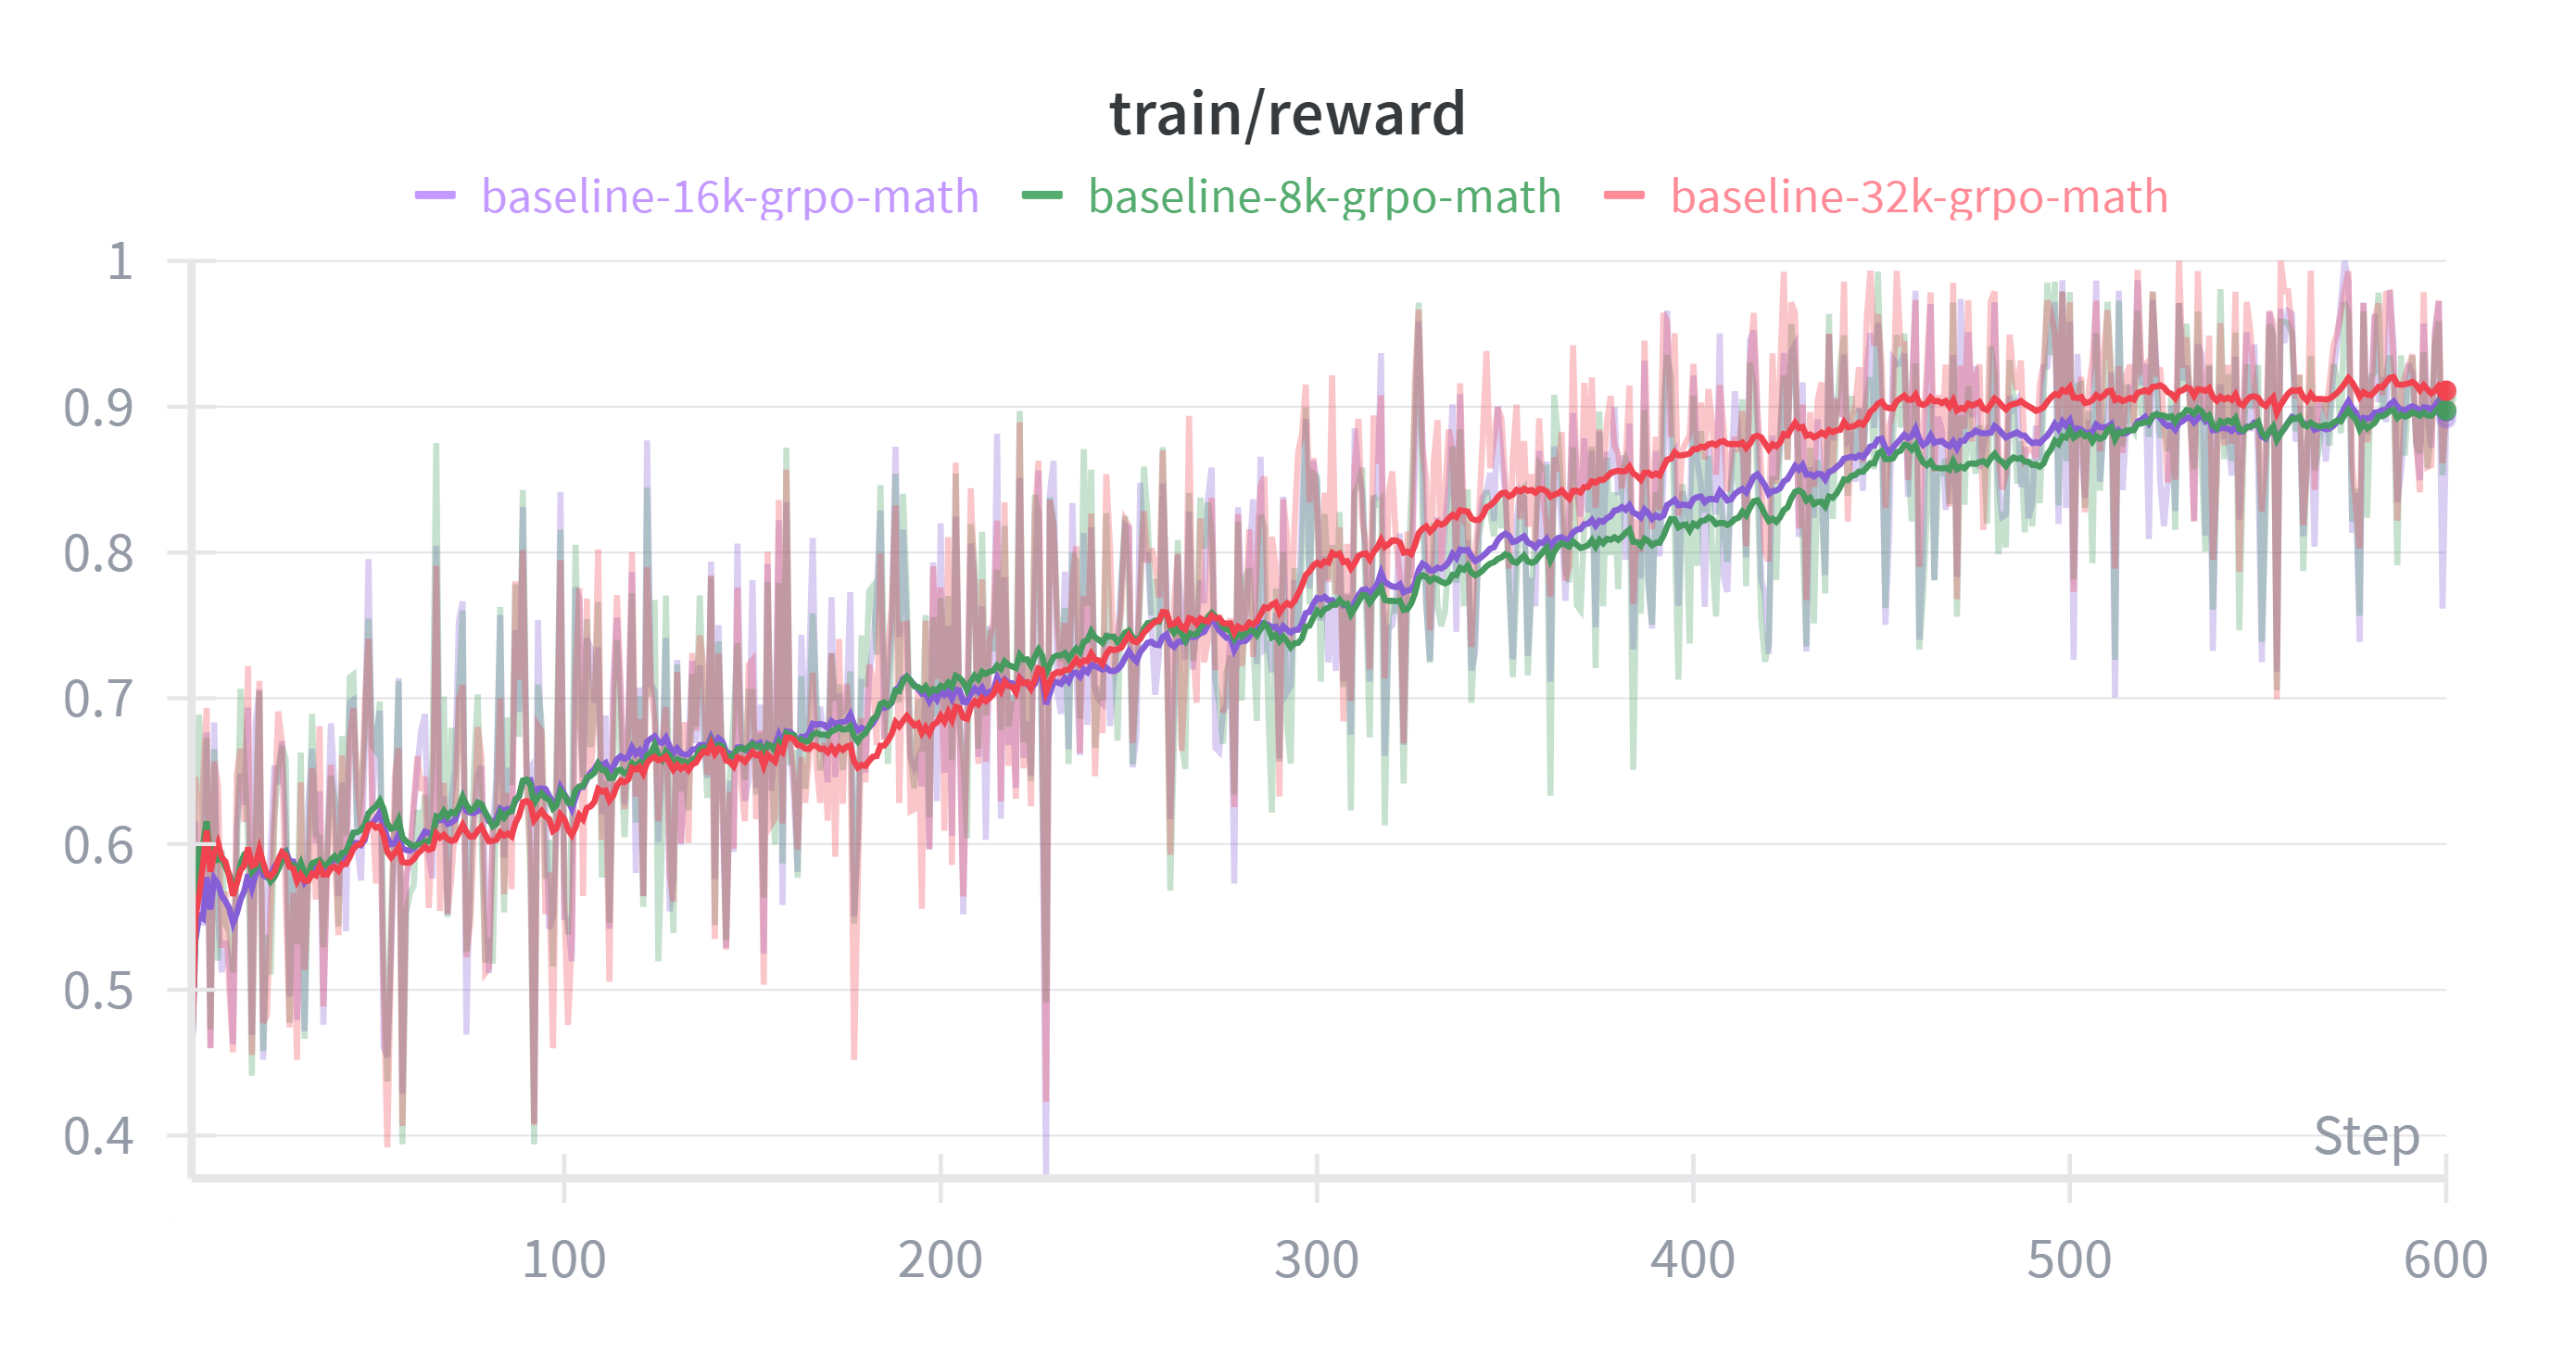
\includegraphics[width=\linewidth]{yarn_reward.png}
\vspace{-2mm}
\caption{YaRNの拡張度合い別のGRPO訓練報酬}
\label{fig:yarn_reward}
\vspace{2mm}
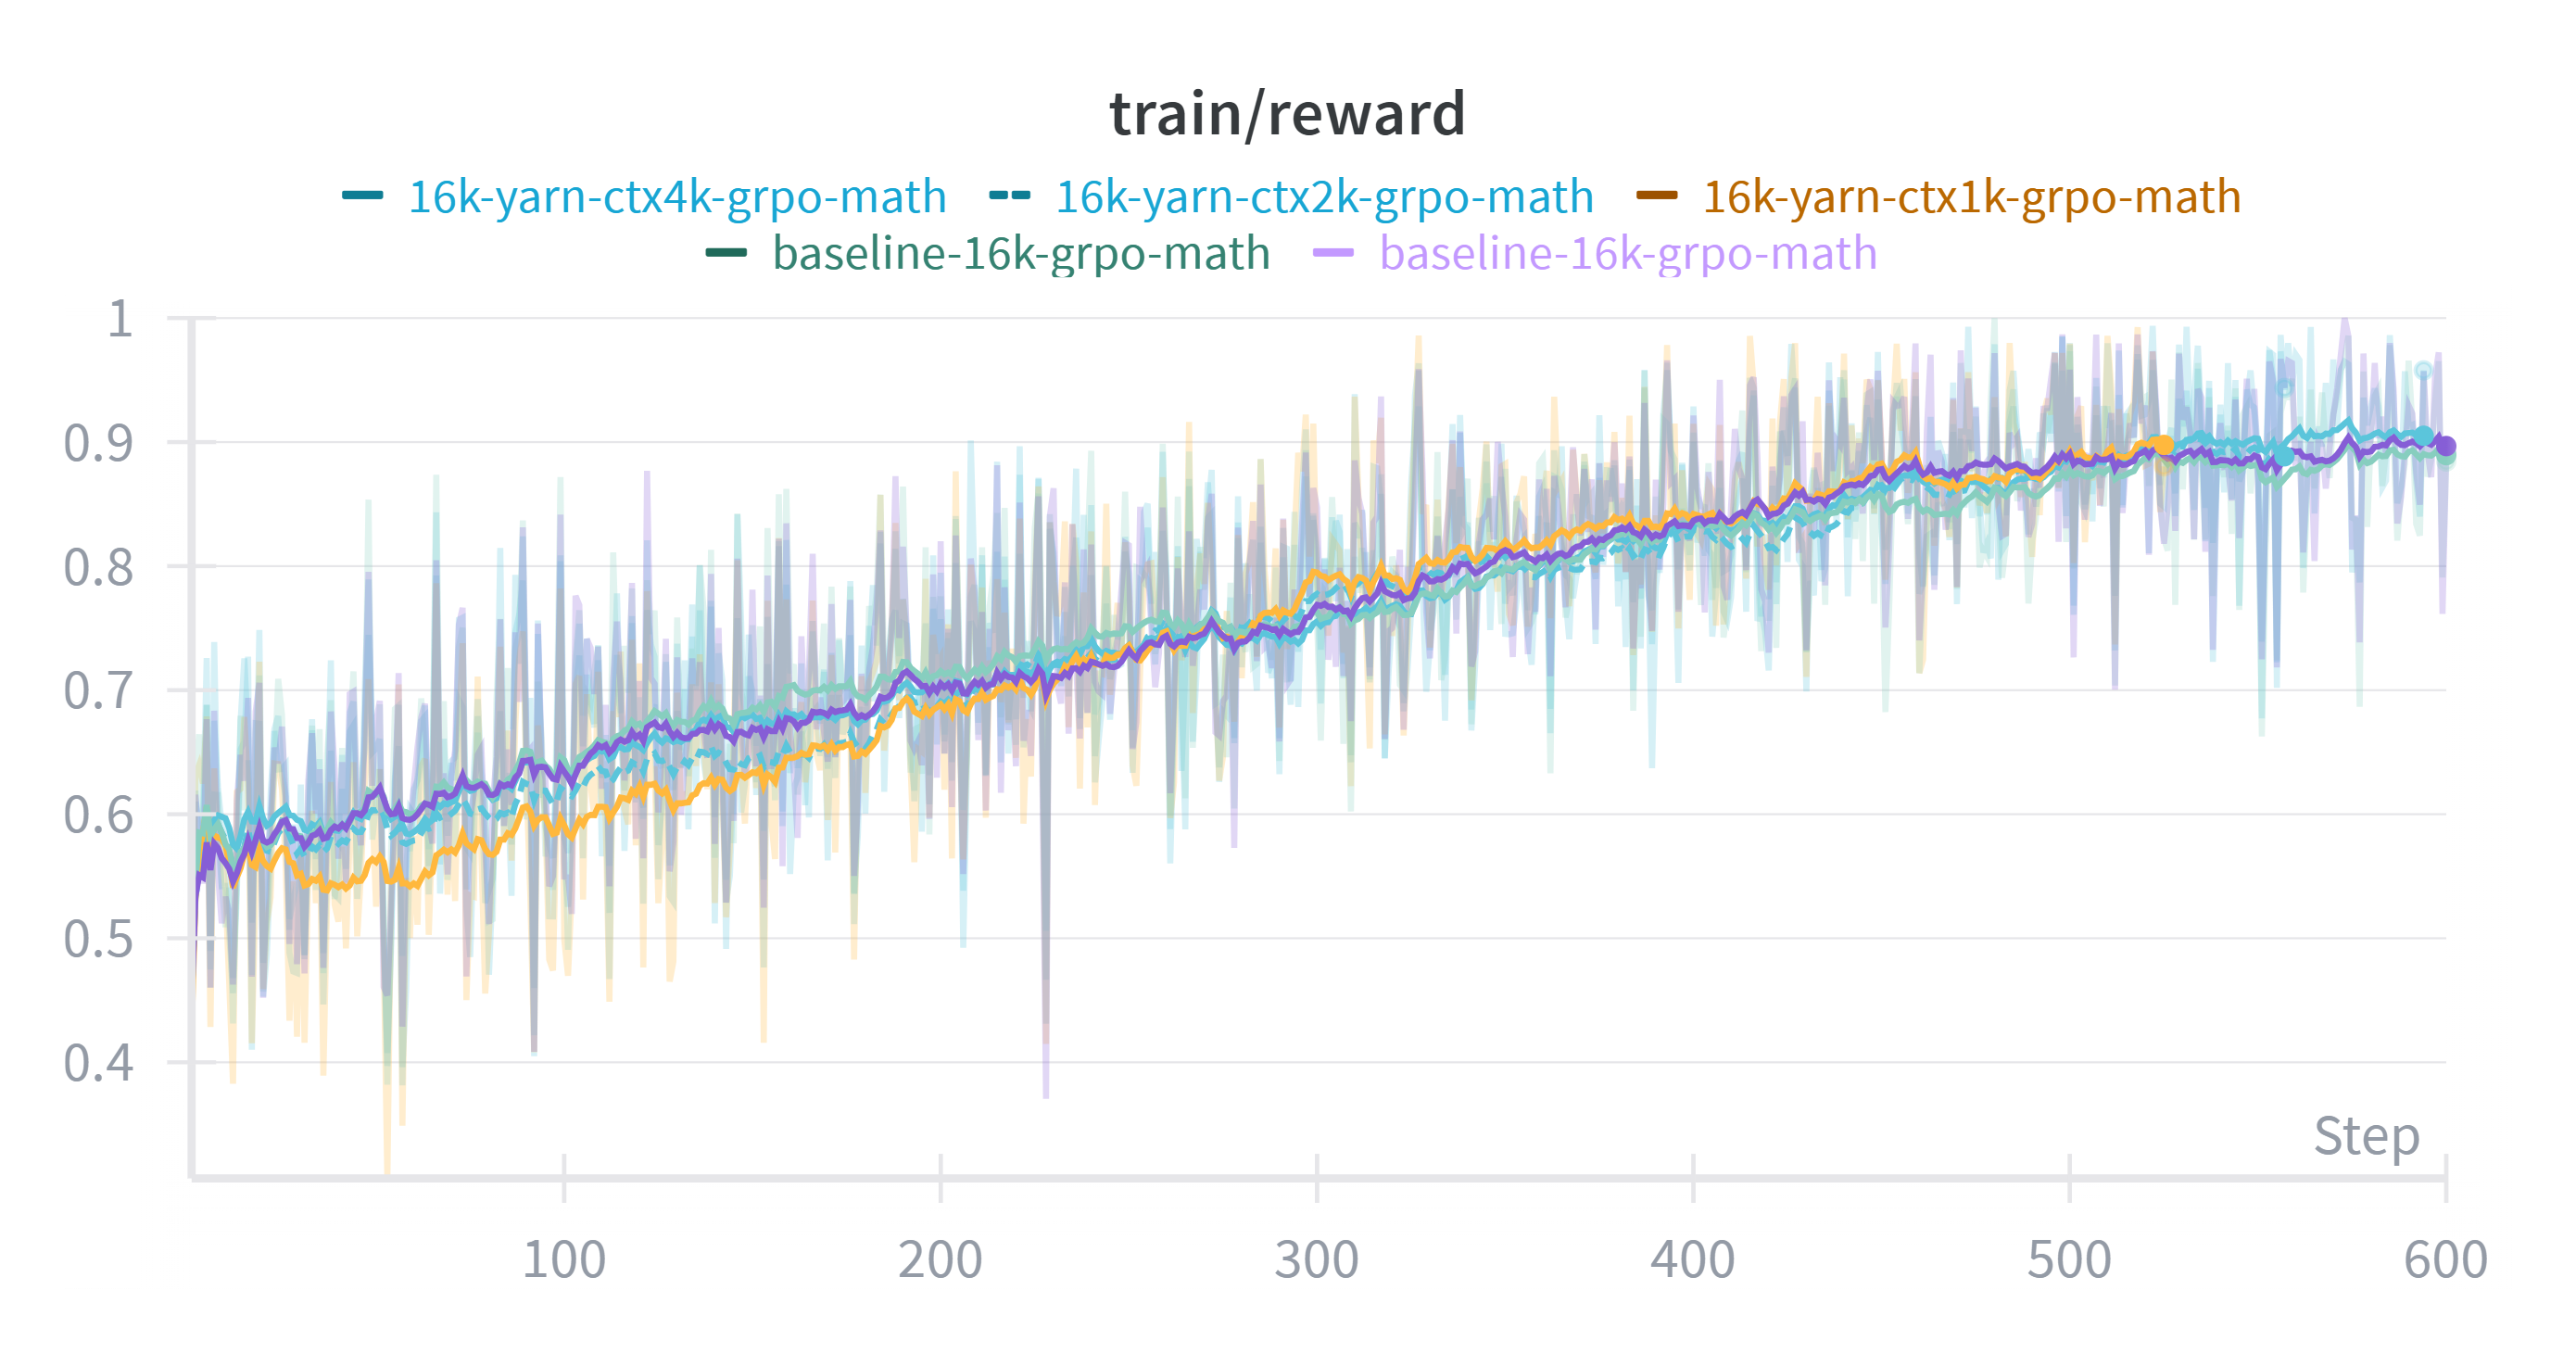
\includegraphics[width=\linewidth]{contextwindow_reward.png}
\vspace{-2mm}
\caption{コンテキストウインドウサイズ別のGRPO訓練報酬}
\label{fig:ctx_reward}
\vspace{2mm}
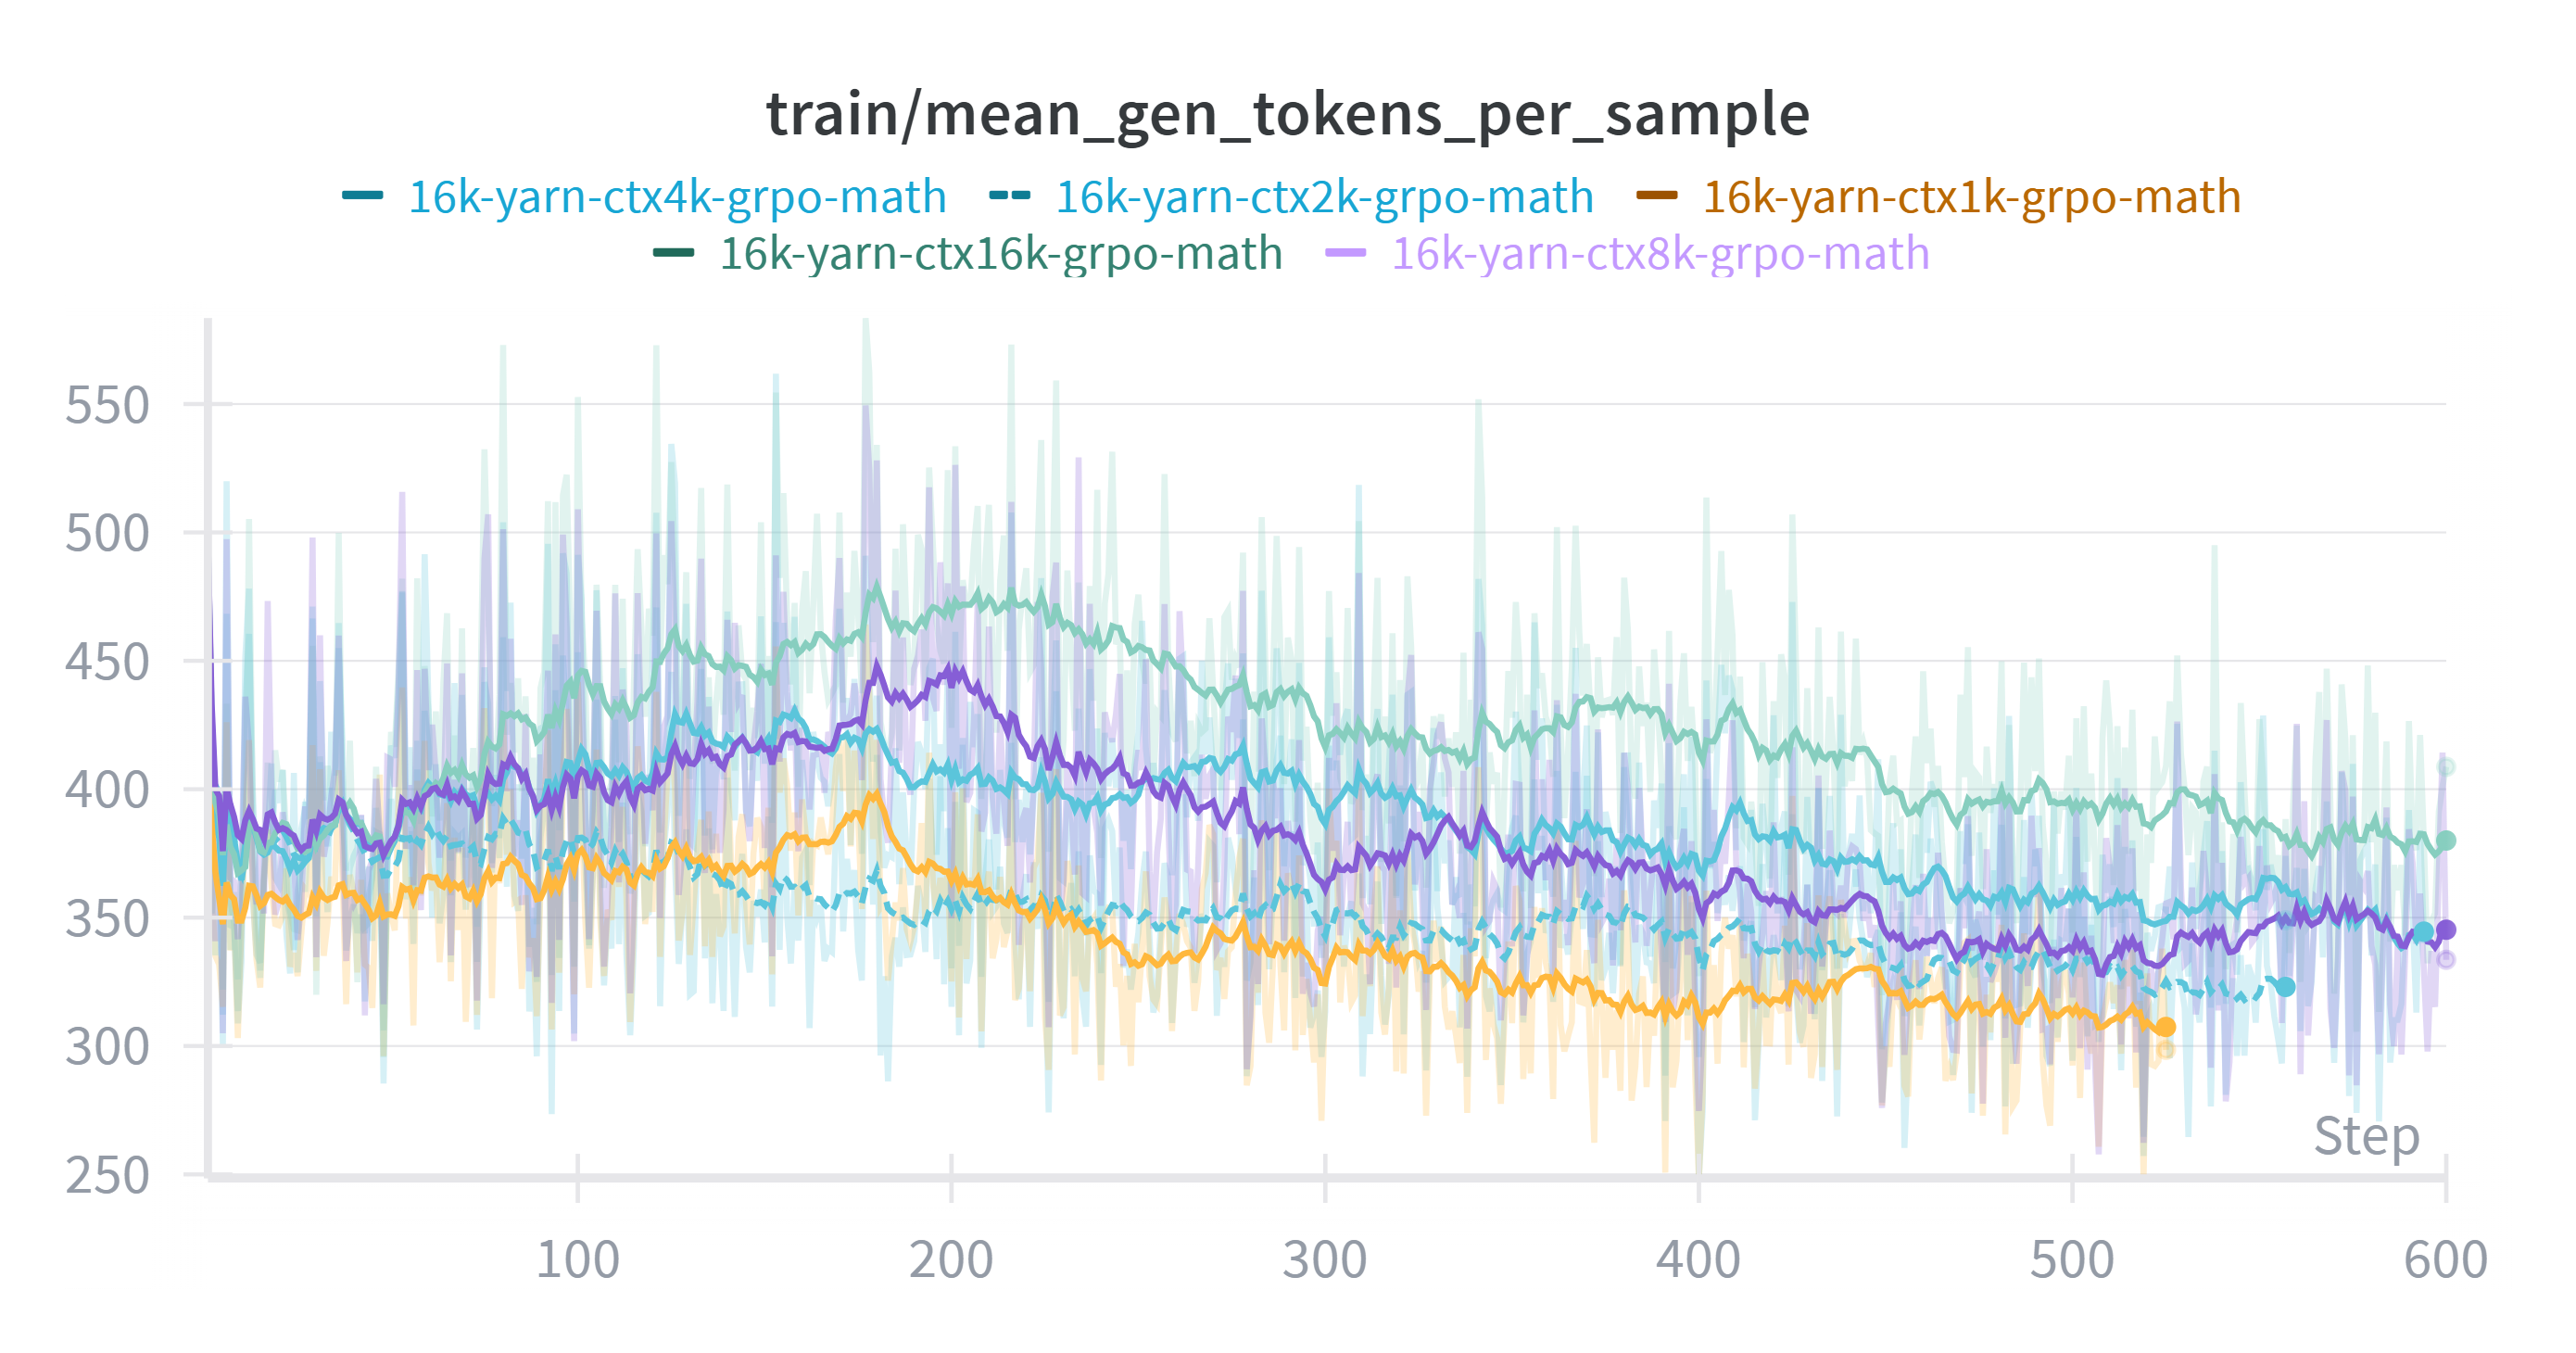
\includegraphics[width=\linewidth]{contextwindow_length.png}
\vspace{-2mm}
\caption{コンテキストウインドウサイズ別の平均生成トークン数}
\label{fig:ctx_length}
\end{figure}

\end{document}
